\documentclass[11pt,a4paper]{article}
\usepackage{ECBEStyle}

\begin{document}

    \begin{labtitlepage}
      {images/adu.png}          % 1: Logo path
      {Experiment Title}        % 2: Title
      {CEN320 -- Lab 3}         % 3: Course Code -- Lab #
      {Student A}               % 4: Student 1
      {Student B}               % 5: Student 2
      {Student C}               % 6: Student 3
      {Eng. Engineer Name}      % 7: Lab Engineer
      {Prof. Professor Name}    % 8: Faculty
    \end{labtitlepage}
    
    \begin{abstract}
        In a lab report, the abstract is a concise summary that gives the reader a quick overview of the entire experiment. It should briefly state the purpose of the experiment and the main objectives being tested or demonstrated. It then outlines the methods used, highlighting the key techniques or approaches without going into procedural detail. Next, it presents the major findings, typically including important quantitative results, trends, or observations. Finally, the abstract should state the overall conclusion, emphasizing whether the objectives were achieved and what the results imply. The entire abstract is usually written in a single paragraph, avoids citations or detailed explanations, and is kept short—often between 150 and 250 words—so that a reader can understand the essence of the work without reading the full report.
        \\\\
        \noindent \textbf{AI use is not allowed in this section.} 
    \end{abstract}
    
    \section{Introduction}
        The introduction of a lab report sets the stage for the experiment by explaining the purpose, objectives, and relevant theoretical background. It should begin by clearly stating what the experiment is designed to demonstrate or investigate, followed by a brief discussion of the scientific principles involved. This is where you present key equations and models that form the basis of the work. For example, Ohm’s law,
        \begin{equation}
            V = IR,
        \label{eq:ohm}
        \end{equation} relates voltage, current, and resistance in an electrical circuit and might serve as the starting point for analyzing measured data. 
        \\\\
        \noindent \textbf{You can use AI to help you write this section, especially for finding sources.} 
    
    \section{Procedure}
        \begin{itemize}
            \item A clear description of the experimental setup, including diagrams or figures if necessary.\\
            \includegraphics[width=0.92\textwidth]{images/setup.png}
        
            \item A hardware schematic with key connections and interfacing information.\\
            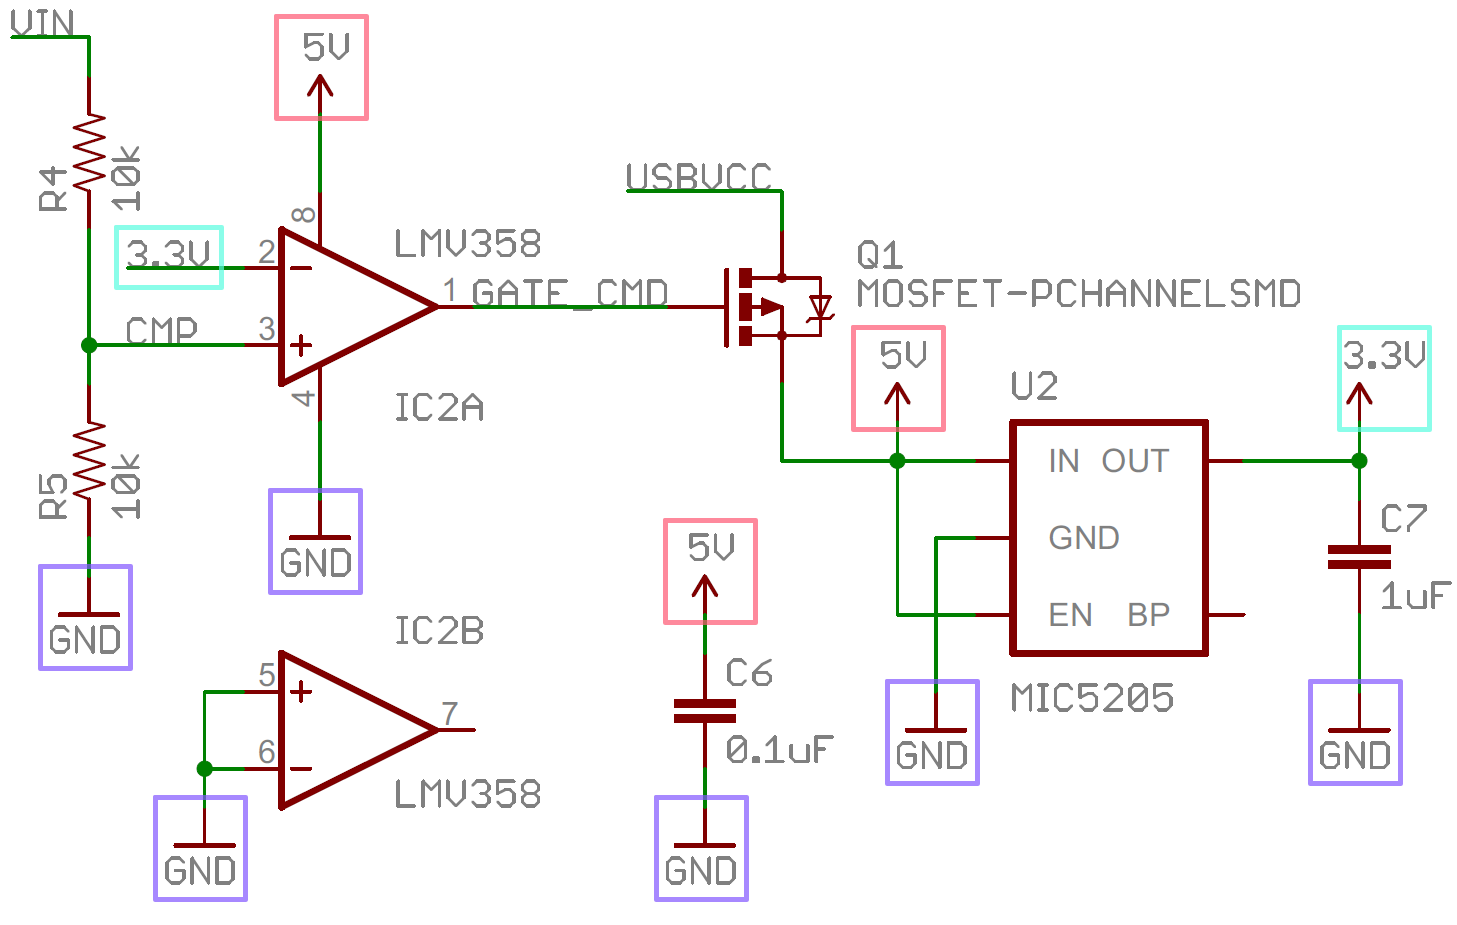
\includegraphics[width=0.92\textwidth]{images/circuit.png}
        
            \item Step-by-step instructions detailing how the experiment was conducted. A picture for each major step.
            \item Information on measurement techniques, calibration procedures, or special precautions taken.
            \item Any variations from the standard procedure or unique conditions applied during the experiment.
            \item Enough detail so that another person could replicate the experiment based solely on this section.
        \end{itemize}
        \noindent \textbf{AI use is not allowed in this section.} 
        
    \section{Results}
        In the Results section of a lab report, you present the data you collected in a clear and organized manner, often using tables (like Table~\ref{tab:example}), graphs, or figures to make trends easy to see. Each table or figure should be referenced in the text and briefly described so the reader understands what it shows without having to interpret it independently. Beyond just presenting raw data, the results section should also include basic analysis, such as calculating derived quantities (e.g., resistance from measured $V$ and $I$ values using Ohm’s law, Eq.~\ref{eq:ohm}), comparing experimental results with theoretical predictions, and identifying any patterns or anomalies. This analysis leads naturally into drawing conclusions—for example, noting whether the measured resistance remained consistent across trials, or whether deviations might be attributed to experimental error, instrument precision, or environmental factors. In short, the Results section is not just about reporting numbers but also about making sense of them, showing how they support (or challenge) the theoretical framework introduced earlier.
        
        The results of the experiment are summarized using tables and figures. All data should be presented clearly and referenced in the text. Tables can be created manually in LaTeX or generated easily using the online tool at \url{https://www.tablesgenerator.com/}, which allows you to copy data from Excel, style the table, and then paste the LaTeX code directly into your report.
    
        \begin{table}[htb!]
          \centering
          \caption{Example measurements.}
          \label{tab:example}
          \begin{tabular}{@{}ccc@{}}
            \toprule
            Trial & $V$ (V) & $I$ (mA) \\
            \midrule
            1 & 2.0 & 1.95 \\
            2 & 3.0 & 2.94 \\
            \bottomrule
          \end{tabular}
        \end{table}
        \noindent \textbf{AI use is not allowed in this section.}     
        
    \section{Conclusion}
        The conclusion of a lab report is a concise section that ties the entire experiment together. It should restate the main objective of the experiment and summarize the most important results without repeating all the details already presented. The focus is on interpreting what the findings mean—whether the objectives were achieved, how well the experimental results aligned with the theoretical expectations, and what the key takeaways are. This is also the place to acknowledge limitations of the experiment, sources of error that may have influenced the results, and suggestions for improving the procedure in future work. Unlike the abstract, which is written as a stand-alone summary, the conclusion directly reflects back on the work in the report, showing how the data and analysis support (or contradict) the intended goals.
        \\\\
        \noindent \textbf{You can use AI to help you write this section, but the interpretation of results and final insights must be your own.} 
    
    \begin{thebibliography}{9}
        \bibitem{smith2020}
        J.~Smith and A.~Lee, ``A simple model for lab reporting,'' \emph{Journal of Educational Labs}, 5(2):123--130, 2020.
    \end{thebibliography}

\end{document}


